\documentclass[tikz,border=8pt]{standalone}
\usepackage{amsmath,amssymb}
\usepackage{tikz}
\usetikzlibrary{angles,quotes}

\begin{document}
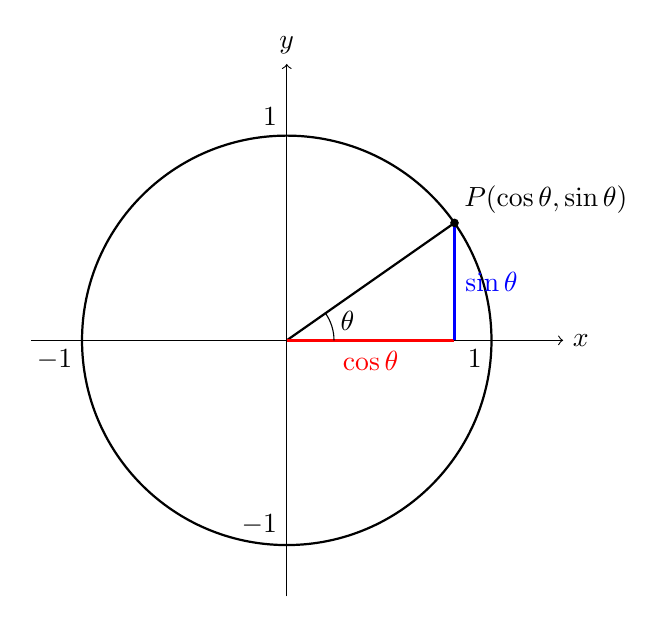
\begin{tikzpicture}[scale=2.6]
  \draw[->] (-1.25,0) -- (1.35,0) node[right] {$x$};
  \draw[->] (0,-1.25) -- (0,1.35) node[above] {$y$};
  \draw[thick] (0,0) circle (1);
  \coordinate (O) at (0,0);
  \coordinate (X) at (1,0);
  \coordinate (P) at (35:1);
  \coordinate (Q) at (35:1 |- O);

  \draw[thick] (O) -- (P);
  \draw[very thick, red]  (O) -- (Q) node[midway, below] {$\cos\theta$};
  \draw[very thick, blue] (Q) -- (P) node[midway, right] {$\sin\theta$};
  \pic[draw, "$\theta$", angle radius=6mm, angle eccentricity=1.35] {angle = X--O--P};
  \fill (P) circle (0.6pt) node[above right] {$P(\cos\theta,\sin\theta)$};

  \foreach \p/\t in {(1,0)/{$1$}, (-1,0)/{$-1$}} \node[below left] at \p {\t};
  \foreach \p/\t in {(0,1)/{$1$}, (0,-1)/{$-1$}} \node[above left] at \p {\t};
\end{tikzpicture}
\end{document}
